\documentclass[pdf]{beamer}
\usepackage{lmodern}
\usepackage[utf8]{inputenc}
\usepackage[estonian]{babel}
\usepackage{eurosym}
\usepackage{tikz}
\usetikzlibrary{patterns}

\usetheme{Madrid}
\setbeamertemplate{navigation symbols}{}

\title[Alglaadur ESTCube-1 kahele moodulile]{Alglaadur ESTCube-1 käsu- ja andmehaldussüsteemile ja kaameramoodulile}
\author{Karl Tarbe}
\institute[]{Matemaatika-informaatikateaduskond}
\begin{document}
\begin{frame}[plain]
    \titlepage
    \centerline{\scriptsize Juhendaja: Meelis Roos}
\end{frame}

\begin{frame}{Toetus}
    \center{
\includegraphics[width=0.9\textwidth]{ITA-logo.jpg}}
\end{frame}
\begin{frame}{Estcube-1}
    \begin{columns}
        \begin{column}{0.5\textwidth}
            \begin{itemize}
                \item 2008, suvi
                \item \(10 \times 10 \times 10\) cm
                \item 1.048 kg
                \item 670 km
                \item 100 000 \euro
            \end{itemize}
        \end{column}
        \begin{column}{0.5\textwidth}
            \center{
\includegraphics[width=\textwidth]{estcube-logo.png}}
        \end{column}
    \end{columns}
\end{frame}

\begin{frame}{Estcube-1}
    \begin{columns}
        \begin{column}{0.5\textwidth}
            \center{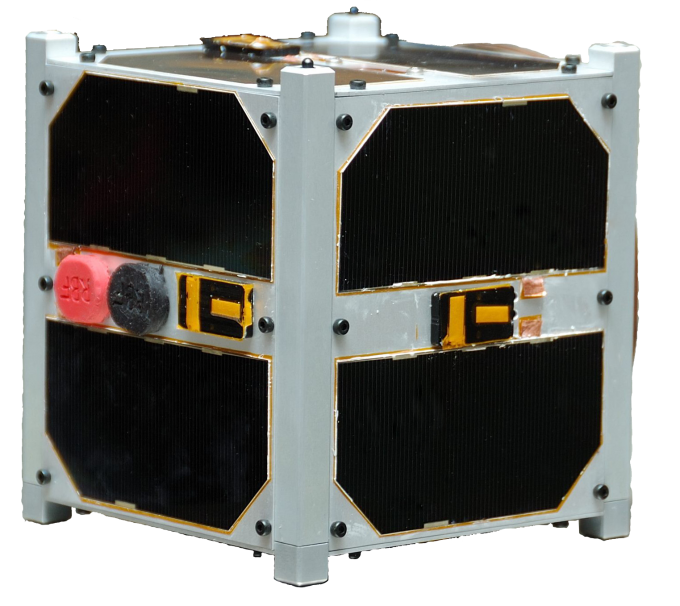
\includegraphics[width=\textwidth]{estcube-photo.png}}
        \end{column}
        \begin{column}{0.5\textwidth}
            \center{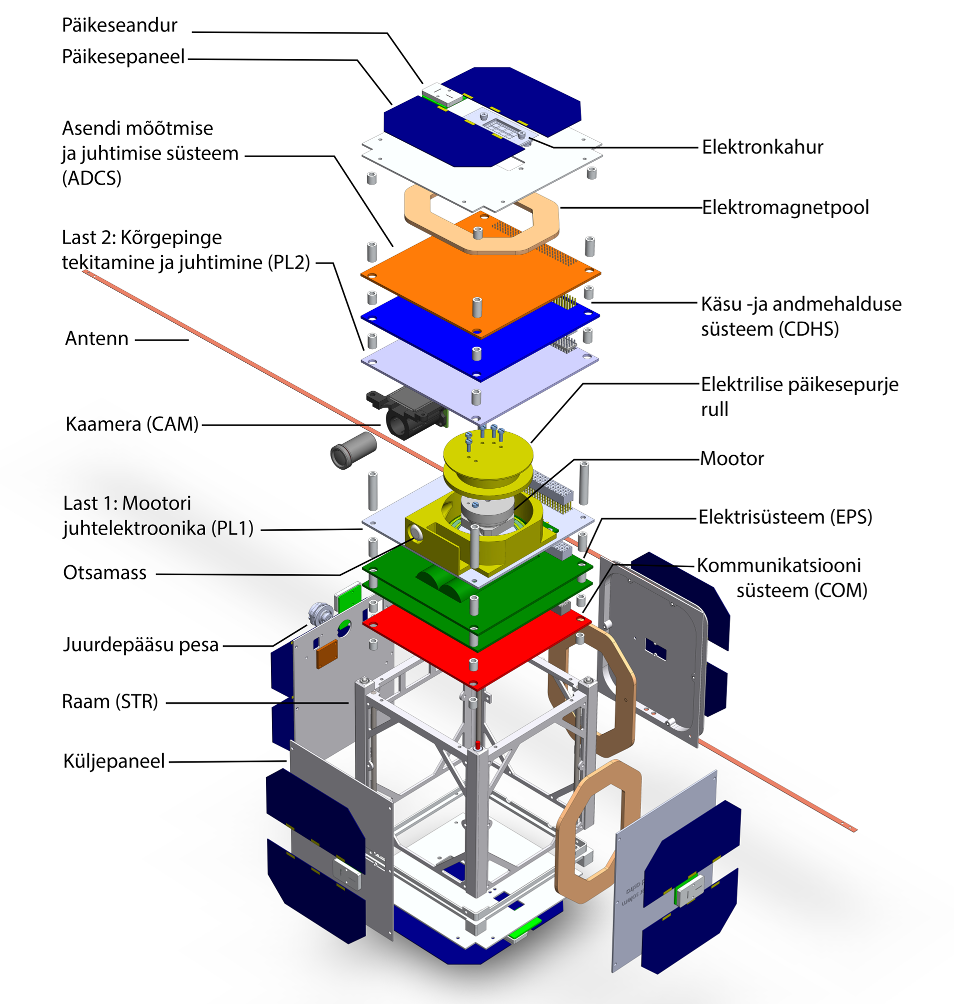
\includegraphics[width=\textwidth]{estcube-assembly.png}}
        \end{column}
    \end{columns}
\end{frame}

\begin{frame}{Käsu- ja andmehaldussüsteem (CDHS)}
    \begin{columns}
        \begin{column}{0.5\textwidth}
            \begin{itemize}
                \item \textit{Command and Data Handling System} \(\to\) CDHS
                \item STM32F103 mikrokontroller (ARM Cortex-M3)
                \item Riistvaraline dubleeritus
                \item FRAM mälud
            \end{itemize}
        \end{column}
        \begin{column}{0.5\textwidth}
            \center{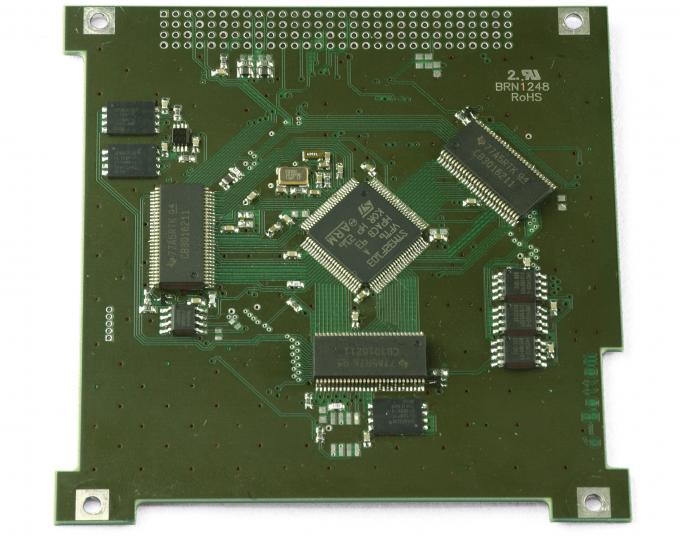
\includegraphics[width=\textwidth]{estcube-CDHS.jpg}}
        \end{column}
    \end{columns}
\end{frame}

\begin{frame}{Kaameramoodul (CAM)}
    \begin{columns}
        \begin{column}{0.5\textwidth}
            \begin{itemize}
                \item STM32F217 mikrokontroller (ARM Cortex-M3)
                \item 640\(\times\)480 
                \item FRAM mälu
            \end{itemize}
        \end{column}
        \begin{column}{0.5\textwidth}
            \center{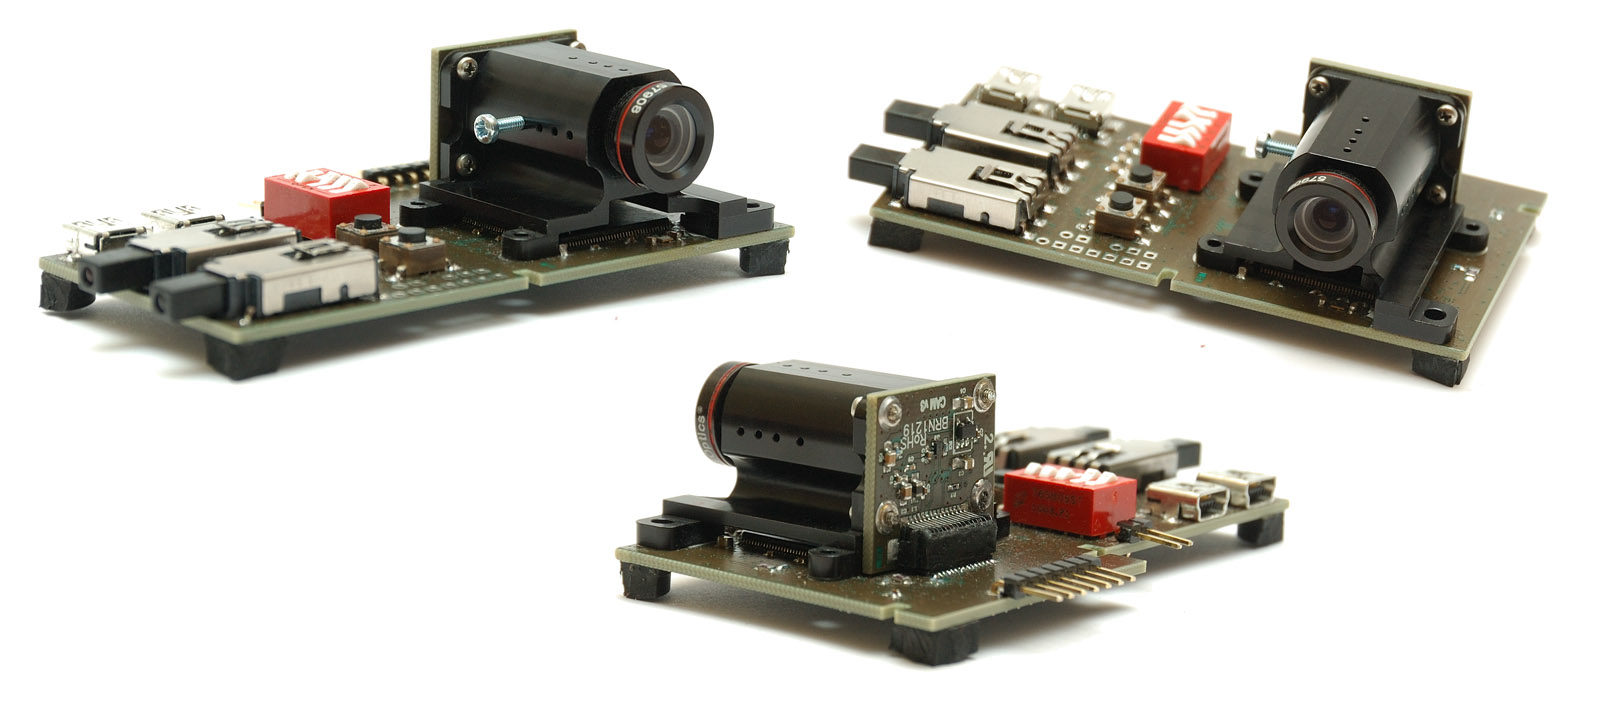
\includegraphics[width=\textwidth]{estcube-CAM.jpg}}
        \end{column}
    \end{columns}
\end{frame}

\begin{frame}{Alglaadur}
    \begin{block}{Ülesanded}
        \begin{itemize}
            \item Tarkvara terviklikkuse kontrollimine
            \item Põhitarkvara uuendamine
            \item Põhitarkvara käivitamine
            \item Tegevuste logi salvestamine
        \end{itemize}
    \end{block}
    \begin{block}{,,Kasutajaliides''}
        \begin{itemize}
            \item Alglaadurile käskude andmine
            \item Tegevuste logi lugemine
        \end{itemize}
    \end{block}
\end{frame}

\begin{frame}{Alglaadur - üldine vaade}
    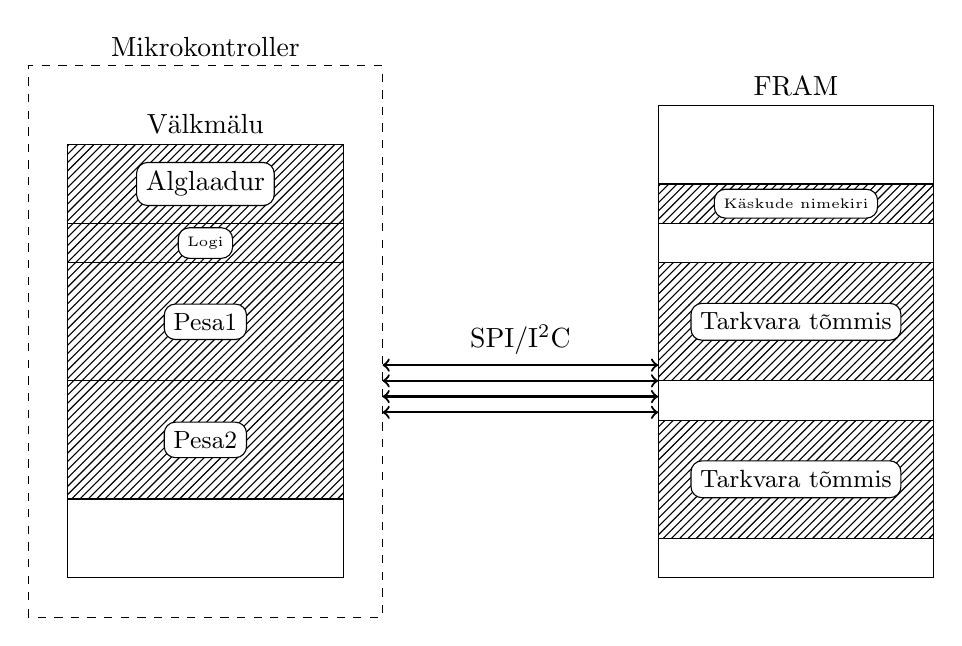
\begin{tikzpicture}
        \draw[dashed] (0,0) rectangle (4.5,7);
        \draw (0.5,0.5) rectangle (4,6);
        \draw (8,0.5) rectangle (11.5,6.5);
        \path (0,7) -- node[above] {Mikrokontroller} (4.5,7);
        \path (0.5,6) -- node[above] {Välkmälu} (4,6);
        \path (8,6.5) -- node[above] {FRAM} (11.5,6.5);

        \draw[pattern=north east lines] (0.5,6) rectangle 
            node[fill=white, draw, rounded corners] {Alglaadur} 
            (4,5);
        \draw[pattern=north east lines] (0.5,5) rectangle
            node[fill=white, draw, rounded corners] {\tiny Logi}
            (4,4.5);
        \draw[pattern=north east lines] (0.5,4.5) rectangle
            node[fill=white, draw, rounded corners] {\small Pesa1}
            (4,3);
        \draw[pattern=north east lines] (0.5,3) rectangle
            node[fill=white, draw, rounded corners] {\small Pesa2}
            (4,1.5);

        \draw[pattern=north east lines] (8,5.5) rectangle
            node[fill=white, draw, rounded corners] {\tiny Käskude nimekiri}
            (11.5,5);
        \draw[pattern=north east lines] (8,4.5) rectangle
        node[fill=white, draw, rounded corners] {\small Tarkvara tõmmis}
            (11.5,3);
        \draw[pattern=north east lines] (8,2.5) rectangle
            node[fill=white, draw, rounded corners] {\small Tarkvara tõmmis}
            (11.5,1);
        \draw[to-to, thick] (4.5,2.6) -- (8,2.6);
        \draw[to-to, thick] (4.5,2.8) -- (8,2.8);
        \draw[to-to, thick] (4.5,3) -- (8,3);
        \draw[to-to, thick] (4.5,3.2) -- node[above]{SPI/I\({}^2\)C} (8,3.2);

    \end{tikzpicture}
\end{frame}

\begin{frame}{Realisatsioon}
    \begin{block}{Märksõnad}
        \begin{itemize}
            \item Madala taseme C
            \item Assembler
            \item \textit{Linker script}
            \item Eclipse
        \end{itemize}
    \end{block}
\end{frame}

\begin{frame}{Mälud}
    \begin{columns}[t]
        \begin{column}{0.46\textwidth}
            \begin{block}{Välkmälu}
                \begin{itemize}
                    \item Asub mikrokontrolleri sees
                    \item Saab muuta lehe kaupa
                    \item Laialt levinud
                    \item Suur andmetihendus
                \end{itemize}
            \end{block}
        \end{column}
        \begin{column}{0.46\textwidth}
            \begin{block}{\textit{Ferroelectric RAM} (FRAM)}
                \begin{itemize}
                    \item Ei asu mikrokontrolleris
                    \item Saab muuta baidi kaupa
                    \item Vähe levinud
                    \item Väike andmetihedus
                \end{itemize}
            \end{block}
        \end{column}
    \end{columns}
\end{frame}

\begin{frame}{SPI ja I\({}^2\)C}
    \begin{columns}
        \begin{column}{0.46\textwidth}
            \begin{block}{\textit{Serial Peripheral Interface}}
                \center{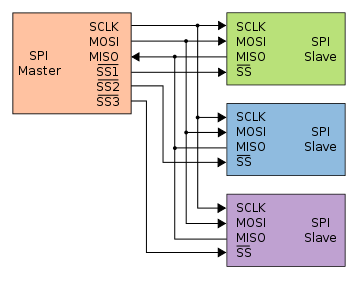
\includegraphics[width=\textwidth]{SPI.png}}
            \end{block}
        \end{column}
        \begin{column}{0.46\textwidth}
            \begin{block}{\textit{Inter-Integrated Circuit}}
                \center{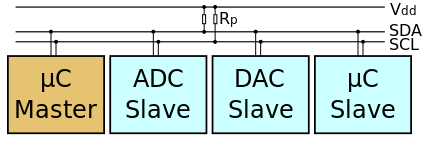
\includegraphics[width=\textwidth]{I2C.png}}
            \end{block}
        \end{column}
    \end{columns}
\end{frame}

\begin{frame}{Tarkvara tervklikkuse kontrollimine}
    \begin{block}{Kuidas kontrollitakse?}
        CRC-32 (Ethernet) polünoom: \( 0x4C11DB7\)
        \[ X^{32} + X^{26} + X^{22} + X^{16} + X^{12}
            + X^{11} + X^{10} + X^8 + X^7 + X^5 + X^4
        + X^2 + X + 1\]
    \end{block}
    \begin{block}{Mida kontrollitakse?}
        \begin{itemize}
            \item Alglaadurit ennast
            \item Kopeerimisel välises mälus olevat tarkvara
            \item Põhitarkvara
        \end{itemize}
    \end{block}
\end{frame}

\begin{frame}{Tarkvara kopeerimine}
    \begin{block}{Töö käik}
        \begin{enumerate}
            \item Käskude nimekirja lugemine
            \item Tarkvara terviklikkuse kontrollimine
            \item Välkmälusse kirjutamine
        \end{enumerate}
    \end{block}
    \begin{block}{Käskude nimekiri}
        \begin{itemize}
            \item Kaks võimalikku käsku
            \item Asub välimises mälus
        \end{itemize}
    \end{block}
\end{frame}

\begin{frame}{Alglaadimine ehk põhitarkvara käivitamine}
    \begin{block}{Töö käik}
        \begin{enumerate}
            \item Tarkvara terviklikkuse kontrollimine
            \item Katkestusvektorite tabeli aadressi seadmine
            \item Stack pointeri seadmine
            \item Lähtestamise vektorile ,,hüppamine''
        \end{enumerate}
    \end{block}
\end{frame}

\begin{frame}{Kokkuvõte}
    \begin{block}{Alglaaduri ülesanded}
        \begin{itemize}
            \item Tarkvara terviklikkuse kontrollimine: \textbf{CRC-32}
            \item Tarkvara kopeerimine: \textbf{FRAM \(\to\) Välkmälu}
            \item Põhitarkvara käivitamine: \textbf{Jump}
        \end{itemize}
    \end{block}
\end{frame}
\end{document}
